\documentclass[tikz,border=0pt]{standalone}
%% Shared style for the figures: TUHH colour palette, Latin Modern fonts.
%% Highlights are bold at caption size (10 pt); longer text is regular and
%% 2 pt smaller (8 pt). Figures are drawn at the text width of the
%% manuscript (390 pt) and must be included unscaled.
\usepackage[T1]{fontenc}
\usepackage{lmodern}
\usepackage{graphicx}
\usepackage{tikz}
\usetikzlibrary{arrows.meta,positioning,calc,fit,backgrounds}

\definecolor{tuhhturquoise}{HTML}{00C1D4}
\definecolor{tuhhyellow}{HTML}{FFDE36}
\definecolor{tuhhred}{HTML}{FF4F4F}
\definecolor{tuhhmint}{HTML}{5AFFC5}
\definecolor{tuhhcoolgray}{HTML}{D0D0CE}
\definecolor{tuhhpurple}{HTML}{7200FE}
\definecolor{tuhhwarmgray}{HTML}{A8968C}
\colorlet{ink}{black!85}

\newcommand{\hl}[1]{{\fontsize{10}{12}\selectfont\bfseries #1}}
\newcommand{\tx}[1]{{\fontsize{8}{9.6}\selectfont #1}}
\newcommand{\txi}[1]{{\fontsize{8}{9.6}\selectfont\itshape #1}}

%% \logo{file stem}{height}{fallback wordmark}: uses logos/<stem>.pdf or
%% .png when present, and a typeset wordmark otherwise.
\newcommand{\logo}[3]{%
  \IfFileExists{logos/#1.pdf}{\includegraphics[height=#2]{logos/#1.pdf}}{%
  \IfFileExists{logos/#1.png}{\includegraphics[height=#2]{logos/#1.png}}{%
  {\fontsize{10}{12}\selectfont\bfseries\sffamily #3}}}}

\tikzset{
  x=1pt, y=1pt, text=ink,
  card/.style={draw=tuhhcoolgray, line width=0.8pt, rounded corners=3pt,
               fill=white},
  band/.style={rounded corners=3pt, draw=none},
  flow/.style={-{Stealth[length=5pt,width=4.5pt]}, line width=1pt,
               draw=ink},
  gap/.style={draw=tuhhred, line width=1pt, dash pattern=on 3pt off 2pt},
  lbl/.style={inner sep=0pt, outer sep=0pt, align=left, anchor=north west},
  tag/.style={fill=tuhhyellow, rounded corners=2pt, inner xsep=3pt,
              inner ysep=1.5pt, anchor=west},
}

\begin{document}
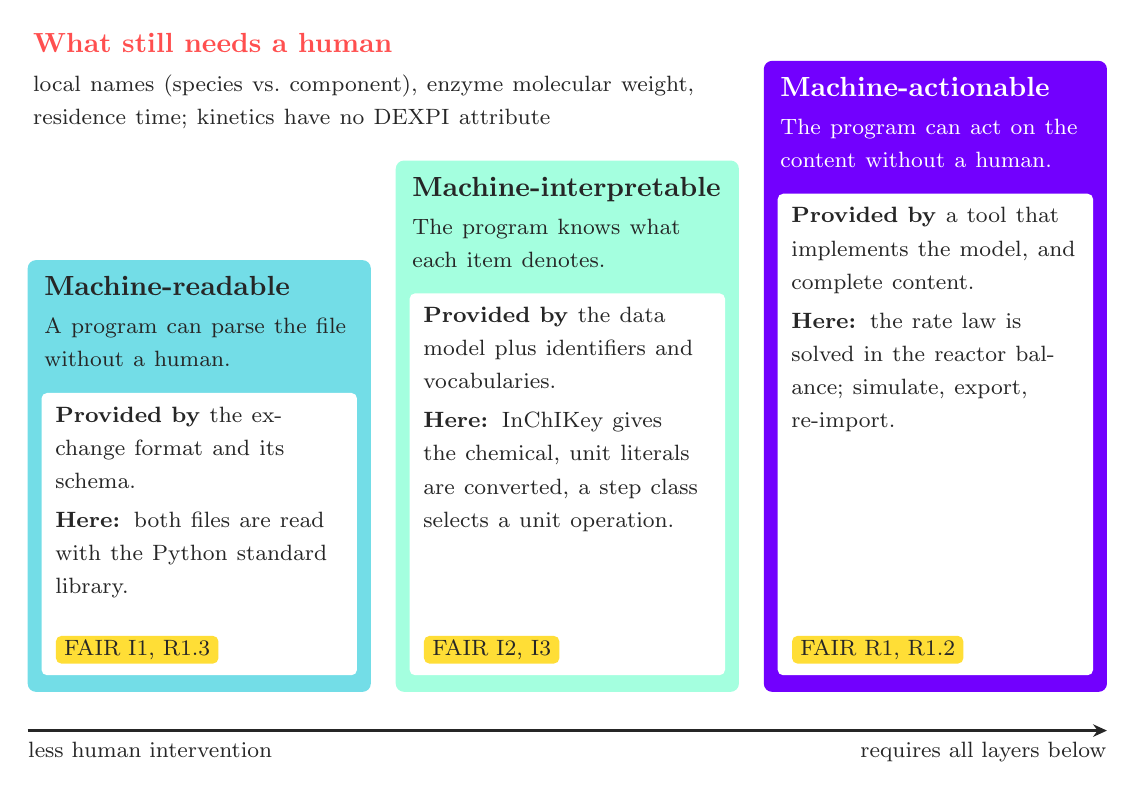
\begin{tikzpicture}
\useasboundingbox (0,0) rectangle (390,268);

% three steps: x 0-124, 133-257, 266-390; rising tops
\newcommand{\step}[9]{%
  \fill[band, #3] (#1,28) rectangle (#1+124,#2);
  \node[lbl, text=#4] at (#1+6,#2-6) {\hl{#5}};
  \node[lbl, text=#4, text width=112pt] at (#1+6,#2-21) {\tx{#6}};
  \fill[white, rounded corners=2pt] (#1+5,34) rectangle (#1+119,#2-48);
  \node[lbl, text width=104pt] at (#1+10,#2-53)
    {\tx{\textbf{Provided by} #7.}\\[2pt]\tx{\textbf{Here:} #8.}};
  \node[tag, anchor=south west] at (#1+10,38) {\tx{FAIR #9}};
}
\step{0}{184}{tuhhturquoise!55}{ink}{Machine-readable}
  {A program can parse the file without a human.}
  {the exchange format and its schema}
  {both files are read with the Python standard library}
  {I1, R1.3}
\step{133}{220}{tuhhmint!55}{ink}{Machine-interpretable}
  {The program knows what each item denotes.}
  {the data model plus identifiers and vocabularies}
  {InChIKey gives the chemical, unit literals are converted,
   a step class selects a unit operation}
  {I2, I3}
\step{266}{256}{tuhhpurple}{white}{Machine-actionable}
  {The program can act on the content without a human.}
  {a tool that implements the model, and complete content}
  {the rate law is solved in the reactor balance; simulate, export,
   re-import}
  {R1, R1.2}

% gaps
\node[lbl, text=tuhhred] at (2,266) {\hl{What still needs a human}};
\node[lbl, text width=250pt] at (2,251)
  {\tx{local names (species vs.\ component), enzyme molecular weight,
       residence time; kinetics have no DEXPI attribute}};

% axis
\draw[flow] (0,14) -- (390,14);
\node[anchor=north west, inner sep=0pt] at (0,10)
  {\tx{less human intervention}};
\node[anchor=north east, inner sep=0pt] at (390,10)
  {\tx{requires all layers below}};
\end{tikzpicture}
\end{document}
